\begin{figure}
\begin{center}
\includegraphics[scale=0.60]{./Figures/Benchmarks.pdf}
\caption{Benchmark suite. Benchmarks with no symbol after their name were taken from the Polybench suite of benchmarks and translated to Chapel. Benchmarks with $\dagger$ are taken from the Chapel Trunk test directory. Benchmarks with $\ddagger$ were developed on our own in order to test specific data access patterns. We also measure the maximum number of elements per follower iterator chunk of work for each benchmark to get a sense of how much aggregation is possible.}
\label{benchmarks}
\end{center}
\end{figure}

\section{Results}\label{sec:results}

To demonstrate the effectiveness of modulo unrolling WU in the Chapel Cyclic and Block Cyclic distributions, we present our results. We have composed a suite of sixteen parallel benchmarks shown in Figure \ref{benchmarks}. Each benchmark is written in Chapel and contains loops with affine array accesses that use zippered iterations, as discussed in Section \ref{sec:array_slicing}. This ensures that the leader and follower iterators where modulo unrolling WU is implemented are called. Our suite of benchmarks contains programs with single, double, and triple nested affine loops. Additionally, our benchmark suite contains programs operating on one, two, and three-dimensional distributed arrays. Thirteen of the sixteen benchmarks are taken from the Polybench suite of benchmarks \cite{polybench} and are translated from C to Chapel by hand. The \textit{stencil9} benchmark was taken from the Chapel source trunk directory. The remaining two benchmarks, \textit{pascal} and \textit{folding}, were written by our group. \textit{pascal} is an additional benchmark other than \textit{jacobi1D} that is able to test Block Cyclic with modulo unrolling WU. \textit{folding} is the only benchmark in our suite that has strided affine array accesses. 

To evaluate improvements due to modulo unrolling WU, we ran our benchmarks using the Cyclic and Block Cyclic distributions from the trunk revision 22919 of the Chapel compiler as well as the Cyclic and Block Cyclic distributions that have been modified to perform modulo unrolling WU, as described in Section \ref{sec:adaptation_in_chapel}. We measure both runtime and message counts for each benchmark. We also compute the geometric means of all normalized runtimes and message count numbers for both distributions to get a sense of how much improvement, on average, modulo unrolling WU provided. 

Data was collected on the ten-locale Golgatha cluster at the Laboratory for Telecommunication Sciences in College Park, Maryland. Each computing node on the cluster is comprised of two 2.93 GHz Intel Xeon X5670 processors, with 24 GB of RAM. The nodes are connected via an InfiniBand network communication link. Benchmarks \textit{fdtd-apml}, \textit{syrk}, \textit{lu}, \textit{mvt}, and \textit{trmm} were run using eight of the ten locales because these programs drew too much power during data collection when all ten locales were used. All other benchmarks were run on ten locales. 

When evaluating modulo unrolling WU used with the Block Cyclic distribution, we only ran two benchmarks (\textit{jacobi-1D} and \textit{pascal}) out of our suite of sixteen because of limitations within the original Chapel Block Cyclic distribution. Many of our benchmarks operate on two or three-dimensional arrays and all require array slicing for the modulo unrolling WU optimization to apply. Both array slicing of multi-dimensional arrays and array slicing containing strides for one-dimensional arrays are not yet supported in the Chapel compiler's Block Cyclic distribution. Implementing such features remained outside the scope of this work. There was no limitation when evaluating modulo unrolling WU with the Cyclic distribution, and all sixteen benchmarks were tested. Once these missing features are implemented in the Chapel compiler, then our method will apply to all of our benchmarks using Block Cyclic.

Figure \ref{runtimes} compares the normalized runtime numbers for the Cyclic and Block Cyclic distributions with and without modulo unrolling WU. For ten out of the sixteen benchmarks, we see reductions in runtime when the modulo unrolling WU optimization is applied to the Cyclic distribution. Both benchmarks tested with the Block Cyclic distribution with modulo unrolling WU show reductions in runtime. On average, modulo unrolling WU results in a 36 percent decrease in runtime for Cyclic and a 53 percent decrease in runtime for Block Cyclic. 

Figure \ref{message_counts} compares the normalized message count numbers for the Cyclic and Block Cyclic distributions with and without modulo unrolling WU. For the Cyclic distribution, nine out of the sixteen benchmarks show reductions in message count 15 percent or greater. Both benchmarks tested with Block Cyclic with modulo unrolling WU show reductions in message count greater than 15 percent. On average, modulo unrolling WU results in a 64 percent decrease in message count for Cyclic and a 72 percent decrease in message count for Block Cyclic. 

The final column in Figure \ref{benchmarks} shows the maximum number of data elements per follower iterator chunk of work for each benchmark. These numbers, measure experimentally, give us a sense of how many data elements can be aggregated into a single message using modulo unrolling WU. Our results show that programs with chunks of work each containing more than a few hundred data elements see a significant runtime and message count improvement when using modulo unrolling WU over the original Chapel distributions. 

\begin{figure}
\begin{center}
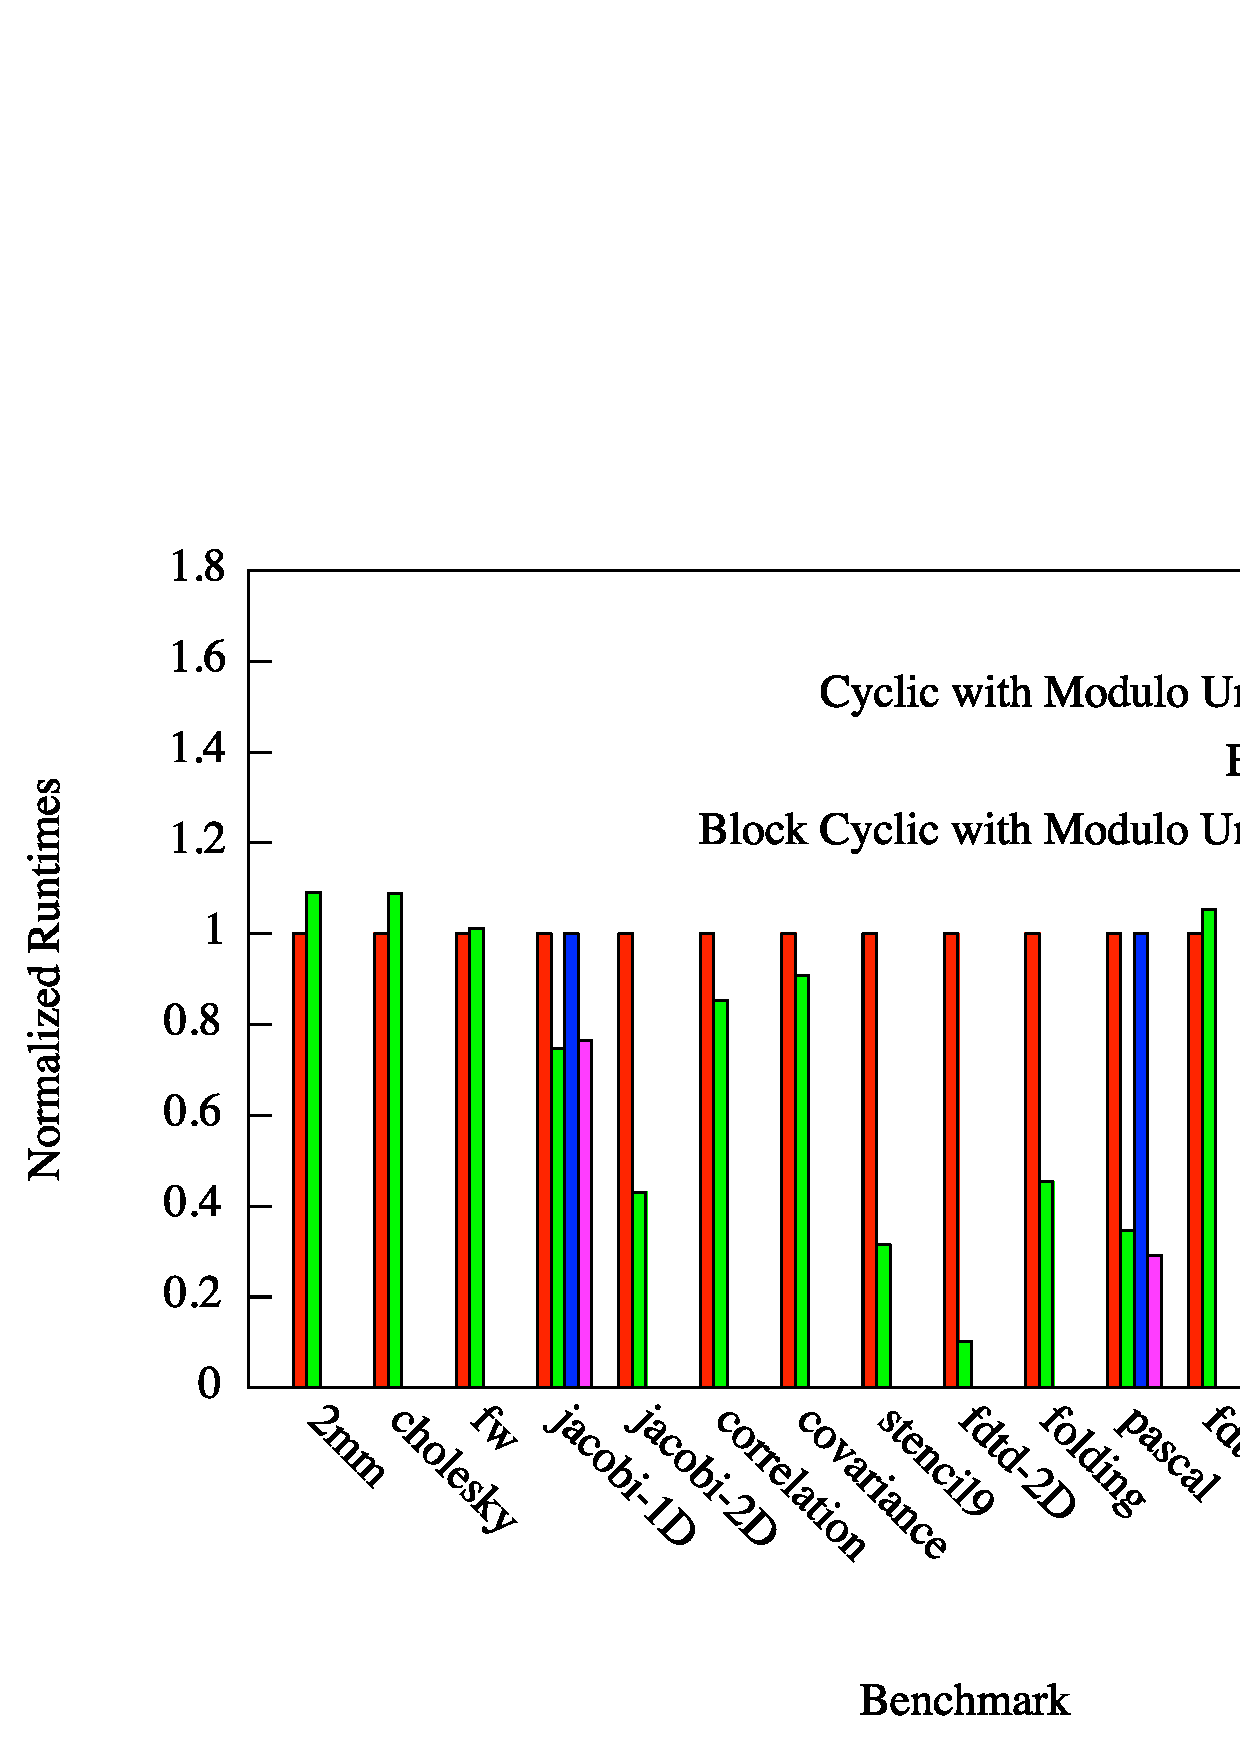
\includegraphics[scale=0.29]{./Figures/runtimes}
\caption{Runtime data collected for our suite of benchmarks. Numbers are normalized to the original Chapel Cyclic and Block Cyclic distributions. }
\label{runtimes}
\end{center}
\end{figure}

\begin{figure}
\begin{center}
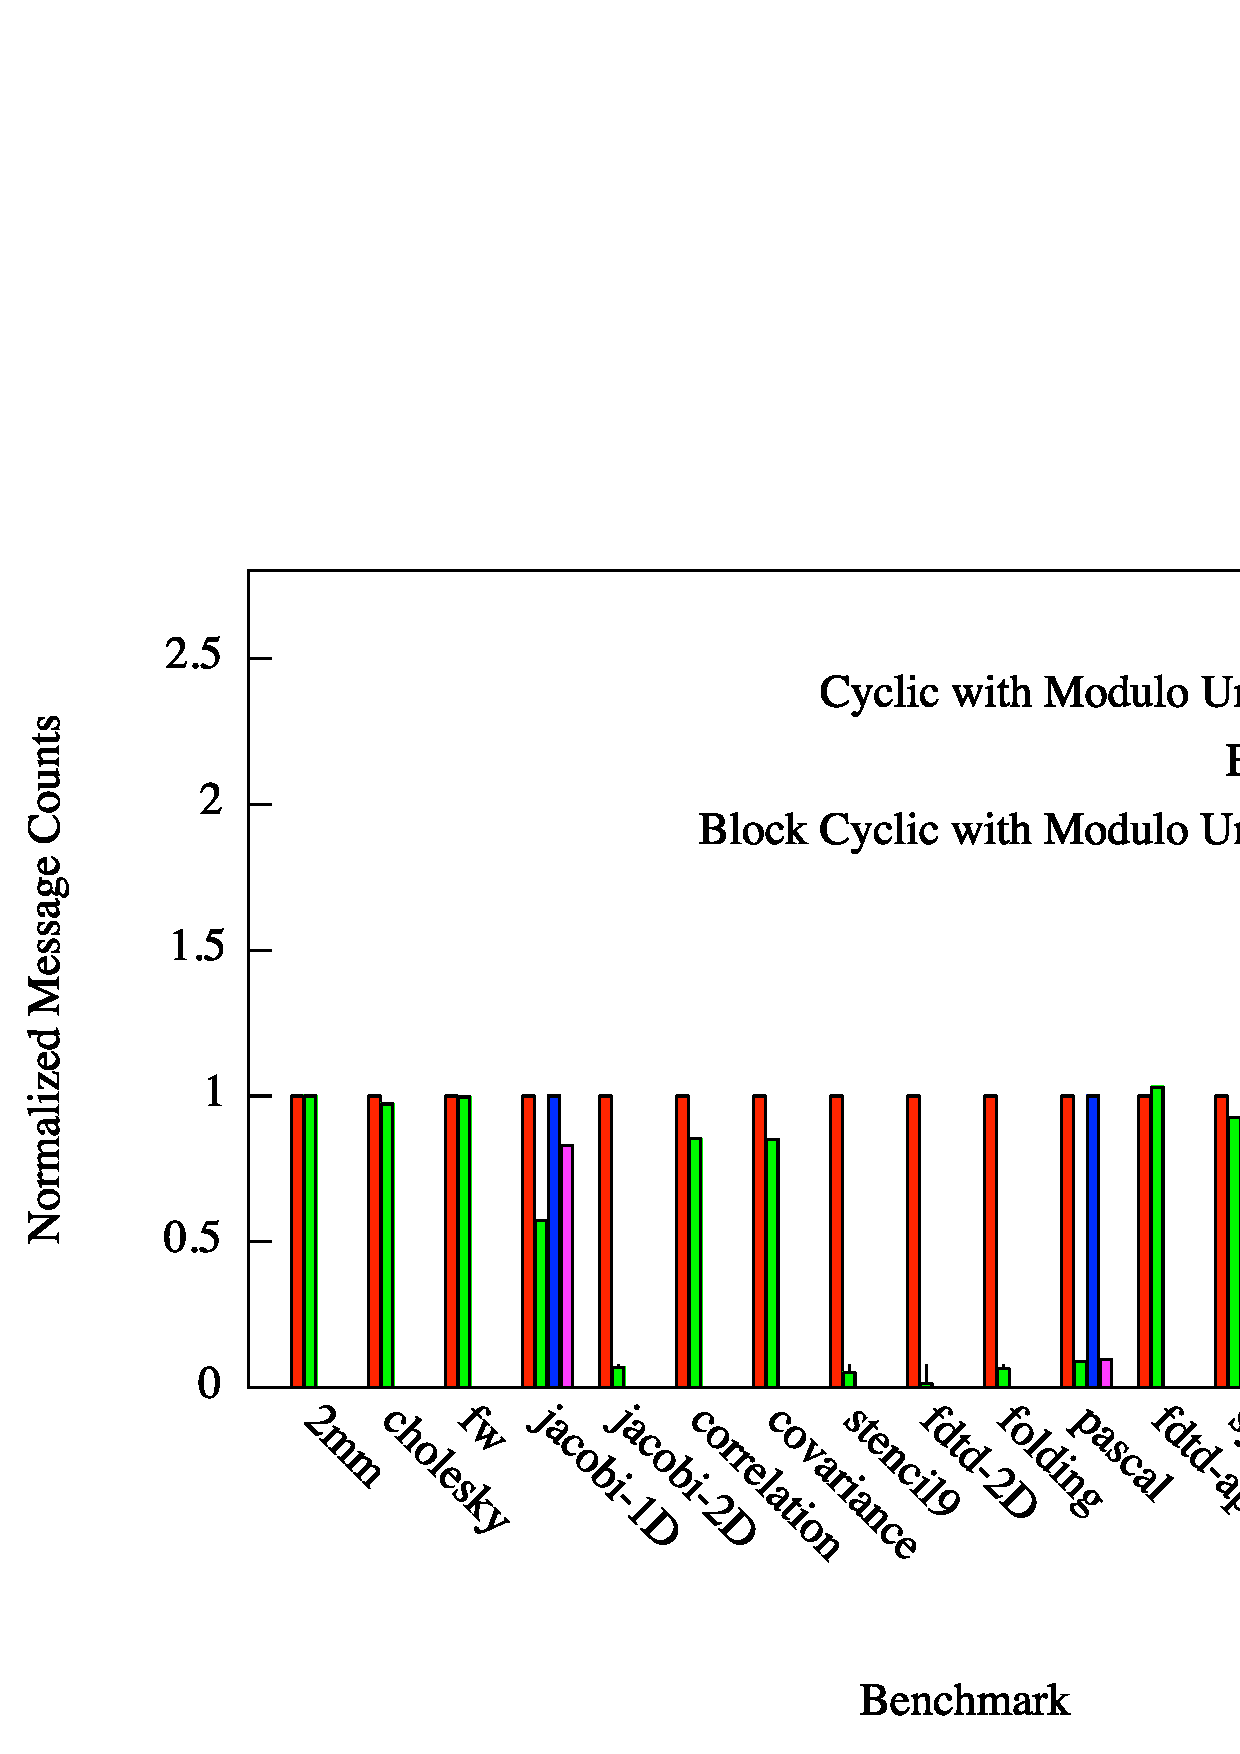
\includegraphics[scale=0.29]{./Figures/message_counts}
\caption{Message count data collected for our suite of benchmarks. Numbers are normalized to the original Chapel Cyclic and Block Cyclic distributions. }
\label{message_counts}
\end{center}
\end{figure}

Some detailed observations on Figures \ref{runtimes} and \ref{message_counts} follow. For six benchmarks that were run using the Cyclic distribution with modulo unrolling WU, runtimes were actually slower and message count numbers either slightly increased or decreased by under 15 percent. Following Figure \ref{benchmarks}, all six of these benchmarks contain follower iterator chunks of work with few data elements. This suggests that, although modulo unrolling WU is applicable to these benchmarks, there is not enough aggregation present within each chunk of work to be worthwhile. For these benchmarks, modulo unrolling WU performs worse because of the optimization's overhead. Unlike normal remote data memory accesses (RDMA), the strided bulk communication primitives \texttt{chpl\_comm\_gets} and \texttt{chpl\_comm\_puts} that are used in the optimization are not hardware optimized and will generally be slower than RDMA when few data elements are being transferred. Furthermore, the Chapel distributions using modulo unrolling WU use more memory than the originals. We yield elements directly from a local buffer within the follower iterator. This could drastically limit the cache performance that we would get when running the original distribution's follower iterator. Our results clearly show that message aggregation using modulo unrolling WU is beneficial for affine programs with large enough parallel chunks of work.

\begin{comment}
\begin{figure}
\begin{center}
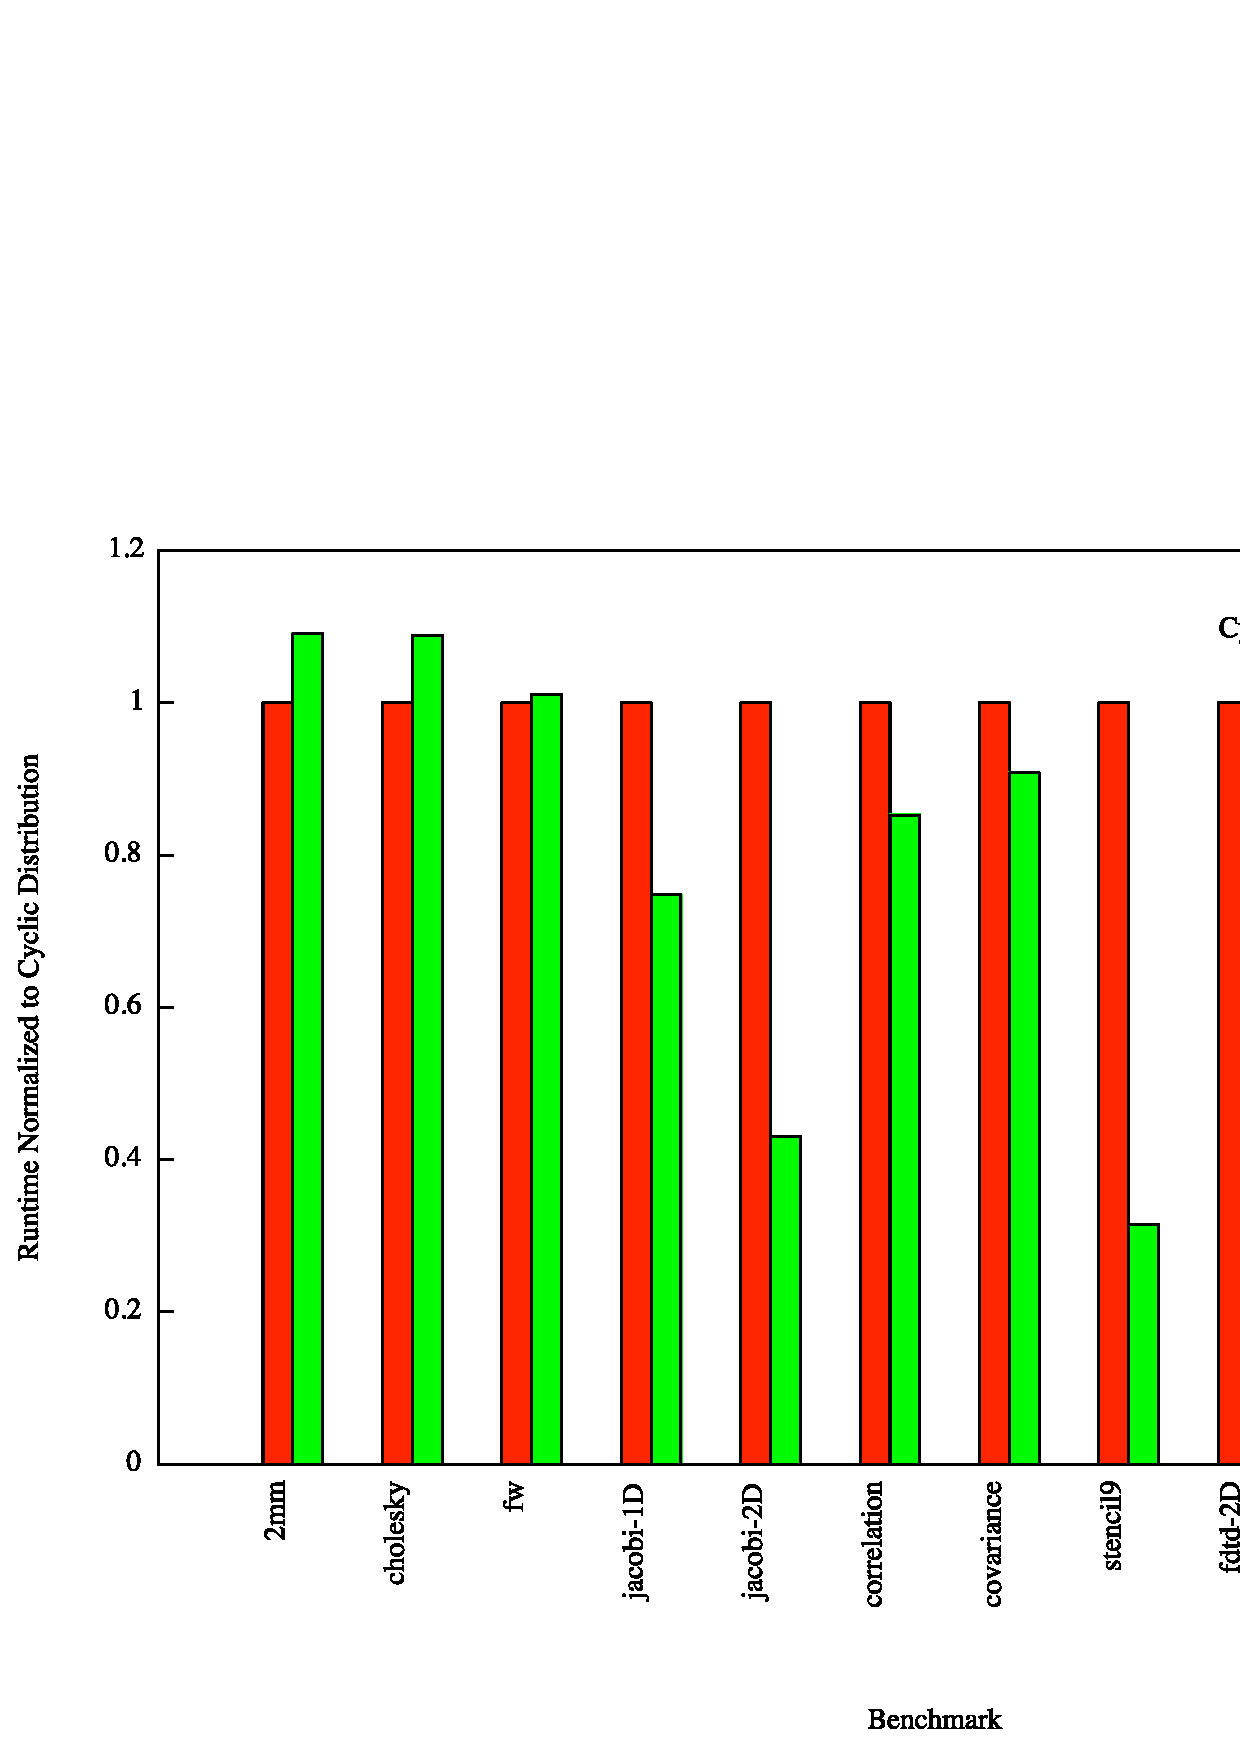
\includegraphics[scale=0.30]{./Figures/cyclic_runtime}
\caption{Cyclic runtime.}
\label{cyclic_runtime}
\end{center}
\end{figure}


\begin{figure}
\begin{center}
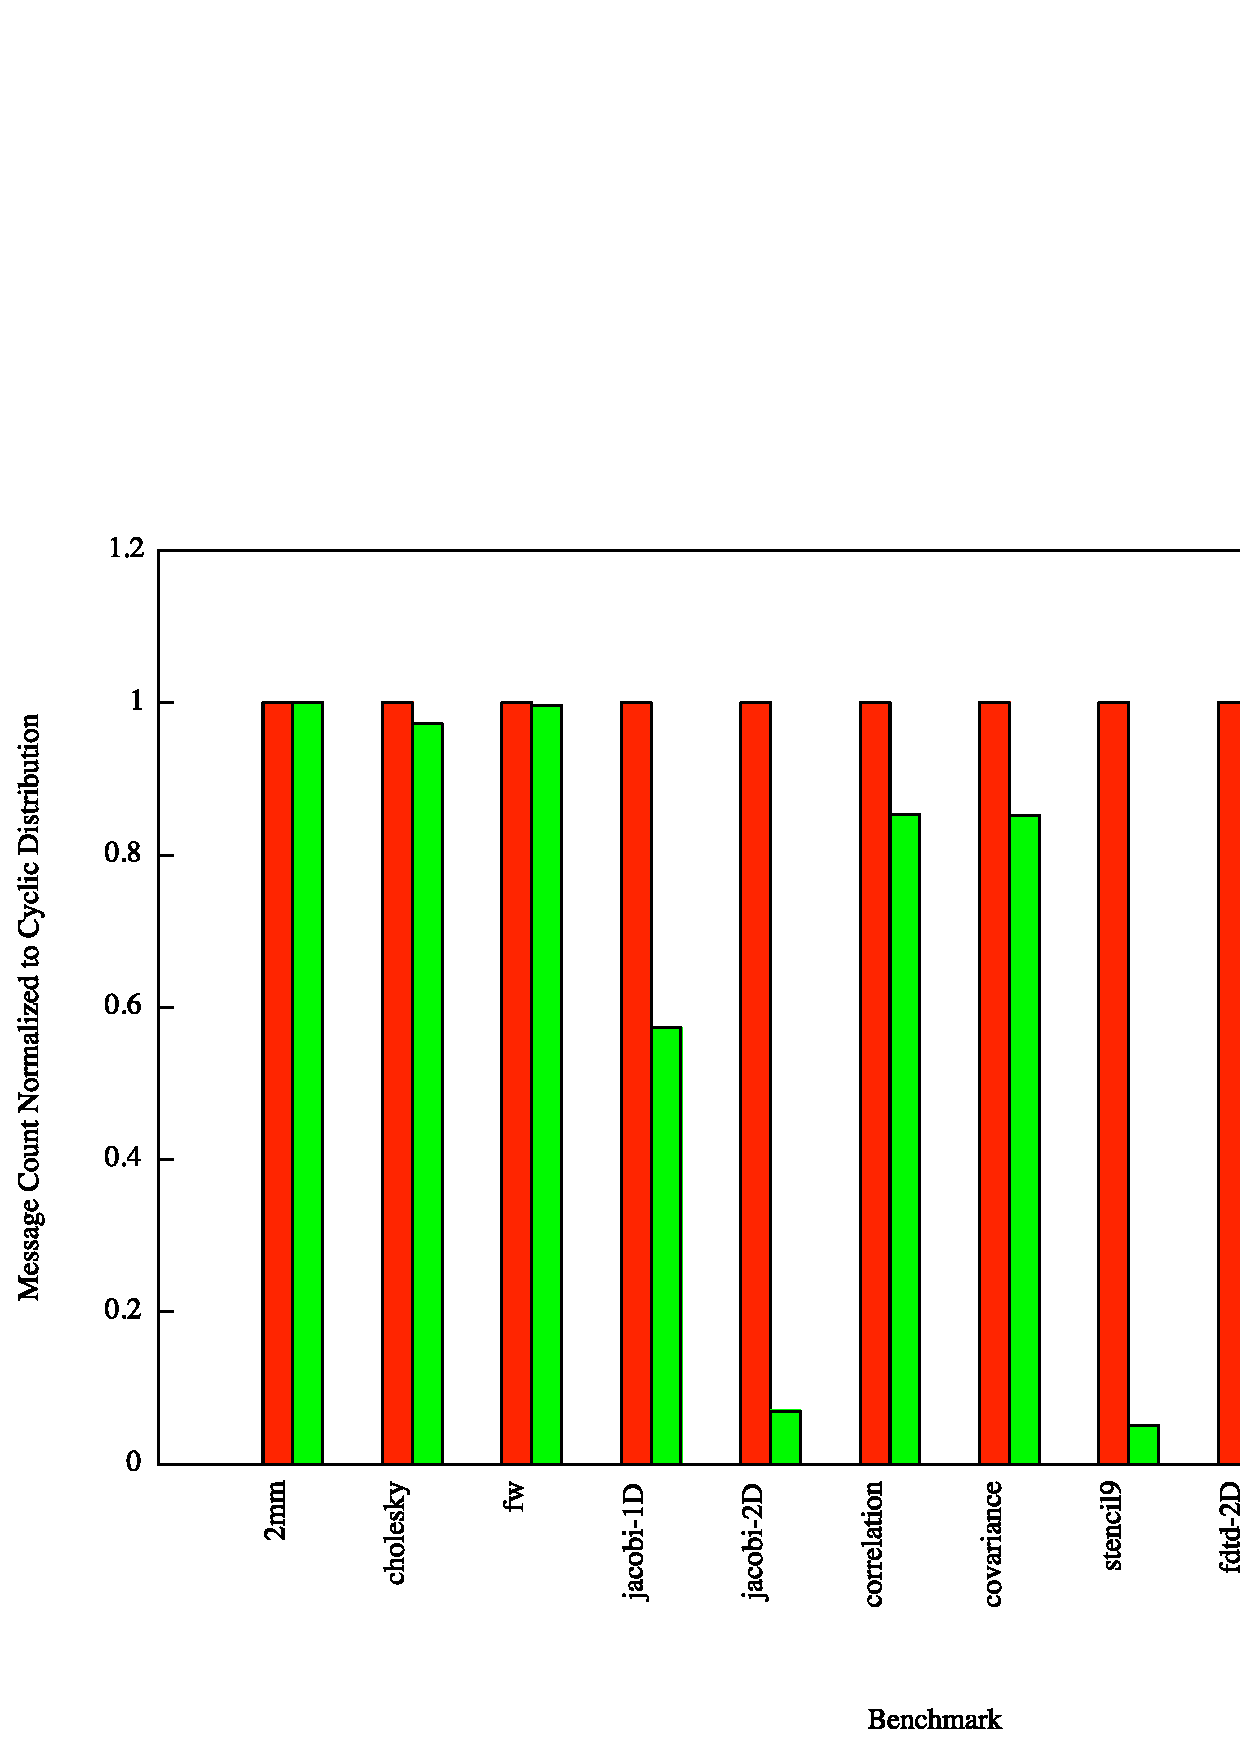
\includegraphics[scale=0.30]{./Figures/cyclic_message_count}
\caption{Cyclic message count.}
\label{cyclic_message_count}
\end{center}
\end{figure}
\end{comment}

\begin{comment}
Figure \ref{runtimes} compare the normalized runtime and message counts respectively for the Cyclic distribution and Cyclic distribution with modulo unrolling WU. For 8 of the 11 benchmarks, we see reductions in runtime when the modulo unrolling WU optimization is applied. On average, modulo unrolling WU results in a 45 percent decrease in runtime. For 9 of the 11 benchmarks, we see reductions in message counts when the modulo unrolling WU optimization is applied. On average, modulo unrolling WU results in 76 percent fewer messages. 

Some detailed observations on Figures \ref{runtimes} and \ref{message_counts} follow. Two of the benchmarks, \textit{cholesky} and \textit{fw}, showed slight improvements in message count when using modulo unrolling WU but did not show improvements in runtime. For the \textit{2mm} benchmark, both runtime and message count did not improve when using modulo unrolling WU. For these benchmarks, the ratio of the problem size to number of locales is not high enough, leading to an insufficient amount of aggregation possible for the computation to see performance improvements. An increase in the number of locales on a system leads to fewer data elements per locale, which naturally means fewer data elements can be aggregated. When this occurs, the cost of performing bulk transfers of a few data elements is more expensive than transferring elements individually. 
\end{comment}

\begin{comment}
\begin{figure}
\begin{center}
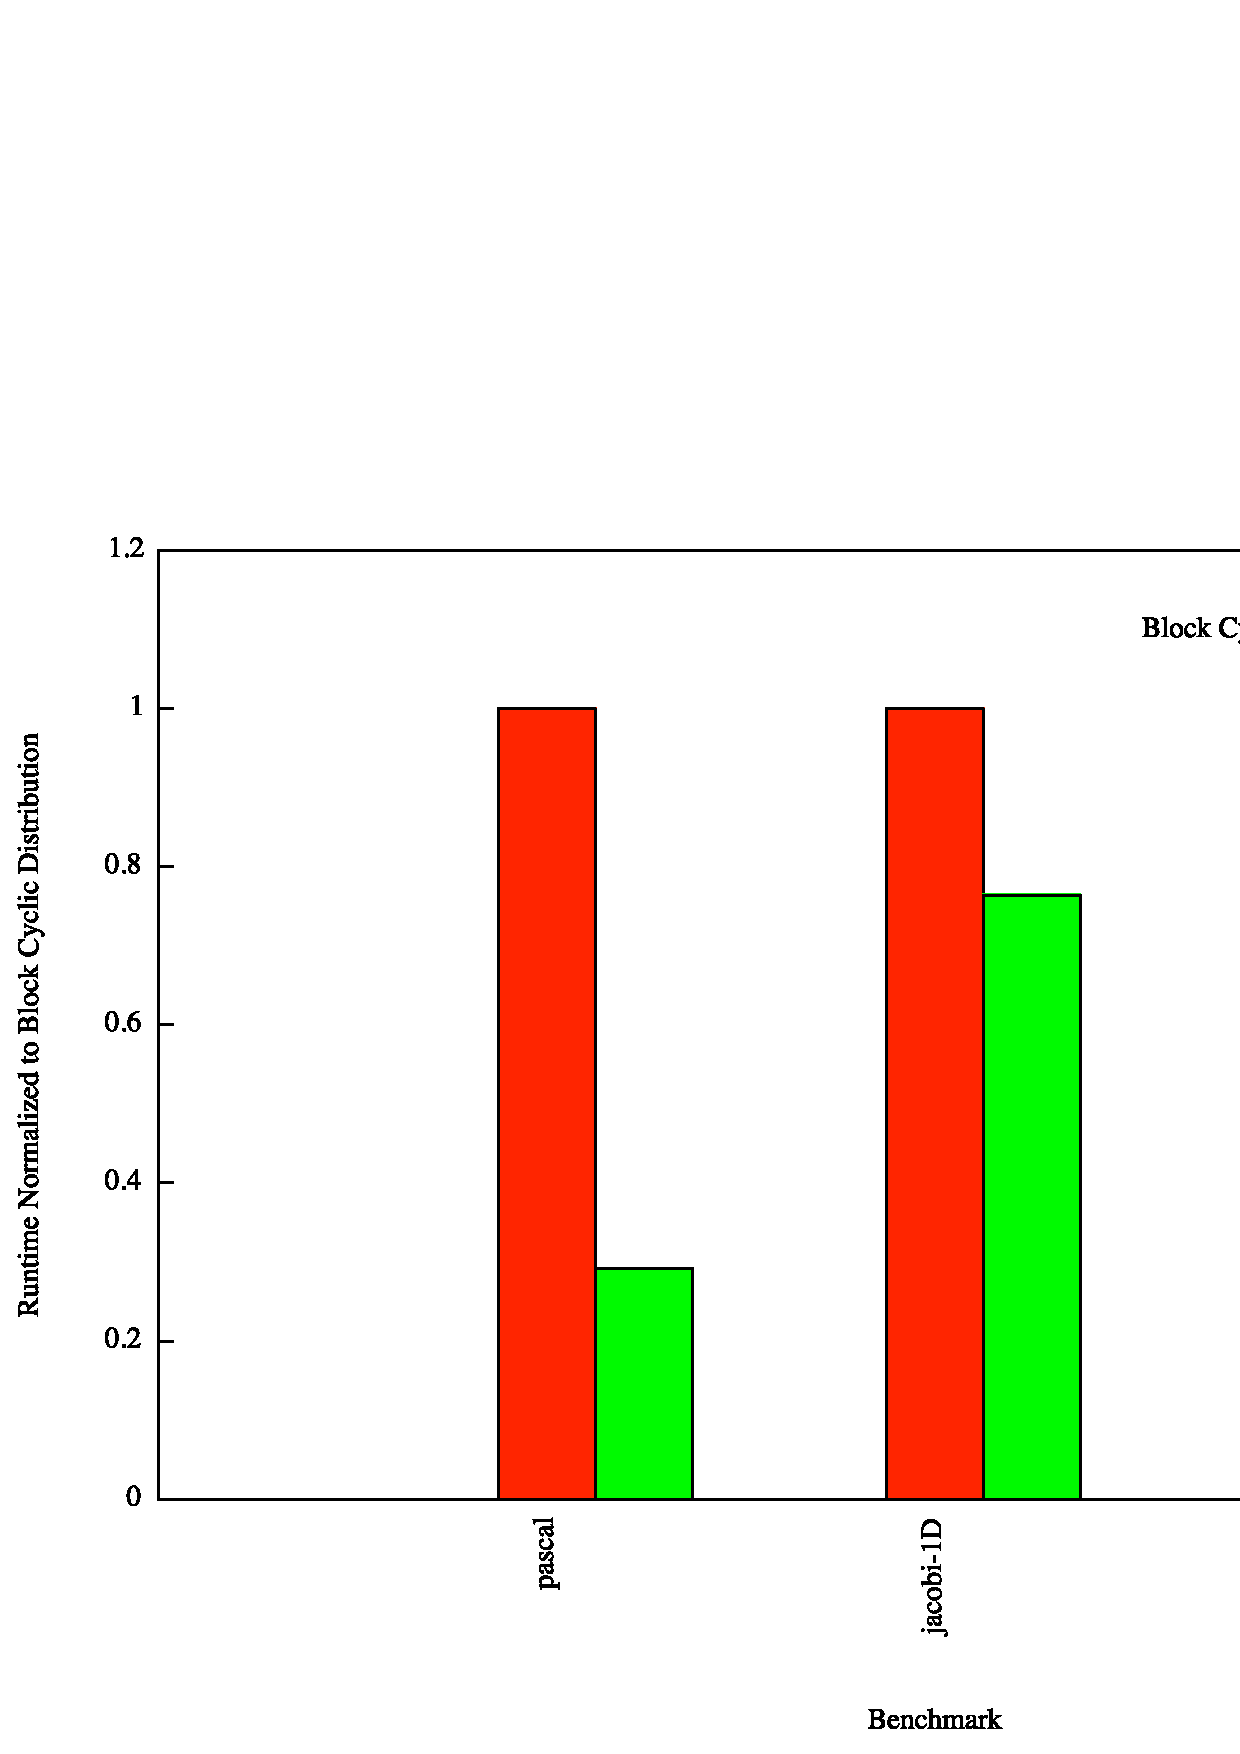
\includegraphics[scale=0.30]{./Figures/block_cyclic_runtime}
\caption{Block Cyclic runtime.}
\label{block_cyclic_runtime}
\end{center}
\end{figure}

\begin{figure}
\begin{center}
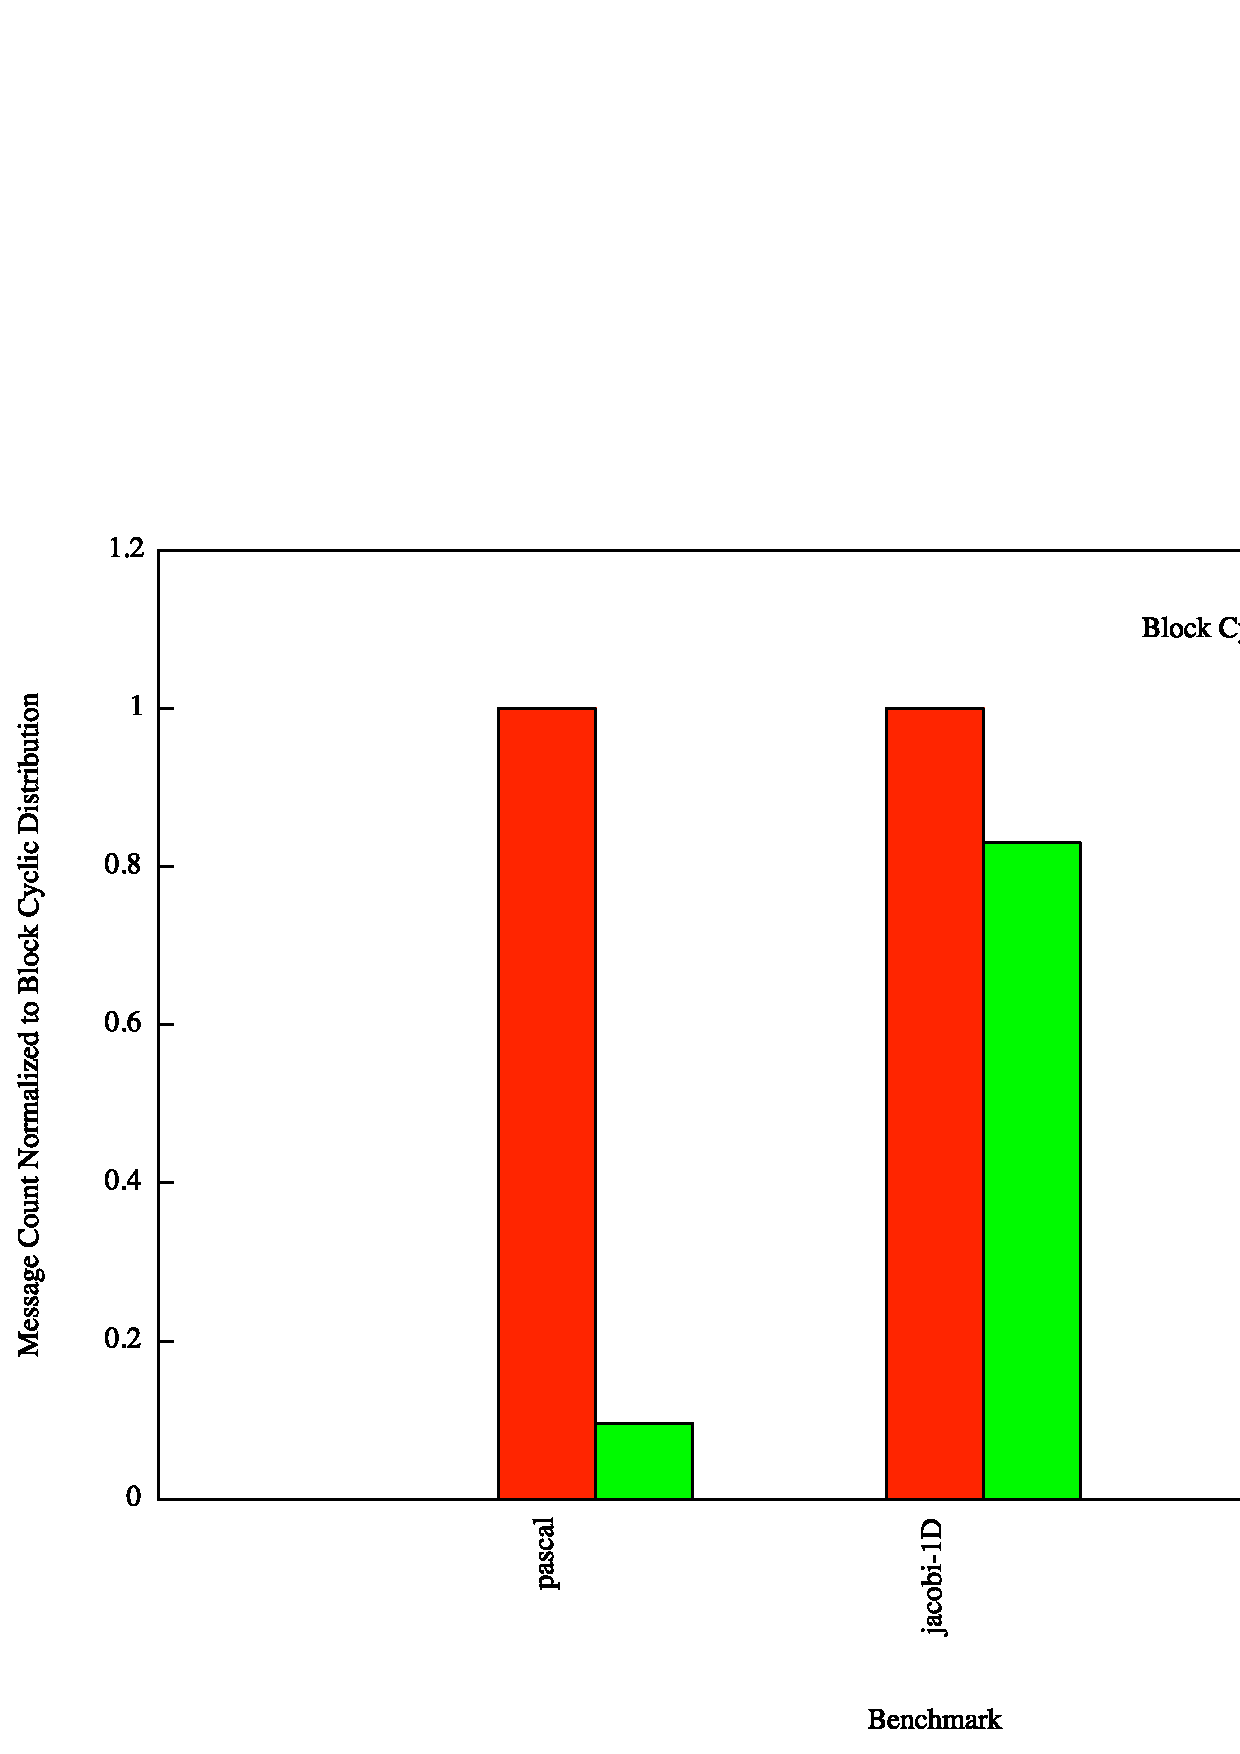
\includegraphics[scale=0.30]{./Figures/block_cyclic_message_count}
\caption{Block Cyclic message count.}
\label{block_cyclic_message_count}
\end{center}
\end{figure}
\end{comment}

\begin{comment}
Figures \ref{block_cyclic_runtime} and \ref{block_cyclic_message_count} compare the normalized runtimes and message counts respectively for the Block Cyclic distribution and Block Cyclic distribution with modulo unrolling WU. For both benchmarks, we see reductions in runtime when the modulo unrolling WU optimization is applied. On average, modulo unrolling WU results in a 52 percent decrease in runtime. For both benchmarks, we see reductions in message counts when the modulo unrolling WU optimization is applied. On average, modulo unrolling WU results in 72 percent fewer messages. 
\end{comment}

